\chapter{Probabilistic Reasoning}

\begin{goals}
\begin{itemize}
    \item See probability as another way to handle uncertainty
    \item Understand how AND and OR work probabilistically
    \item Compare with fuzzy logic
    \item Notice the algebraic pattern
\end{itemize}
\end{goals}

\section{Probability vs Fuzziness}

Fuzzy: ``The water is 0.7 hot'' (degree of truth)

Probabilistic: ``There's 0.7 probability the water is hot'' (uncertainty about a crisp fact)

Different interpretations, but similar math.

\section{Probabilistic Connectives}

For independent events $A$, $B$ with probabilities $p$, $q$:

\textbf{Conjunction}:
\[
P(A \land B) = P(A) \cdot P(B) = p \cdot q
\]

\textbf{Disjunction} (inclusive):
\[
P(A \lor B) = P(A) + P(B) - P(A \land B) = p + q - pq
\]

\textbf{Negation}:
\[
P(\neg A) = 1 - P(A) = 1 - p
\]

\section{Example: Probabilistic Inference}

Consider a simple Bayesian network:
\begin{center}
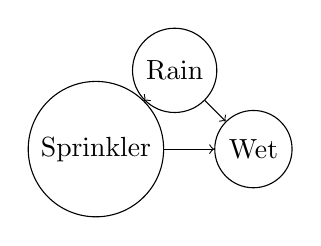
\begin{tikzpicture}
\node[circle, draw] (R) at (0,1) {Rain};
\node[circle, draw] (S) at (-1,0) {Sprinkler};
\node[circle, draw] (W) at (1,0) {Wet};
\draw[->] (R) -- (S);
\draw[->] (R) -- (W);
\draw[->] (S) -- (W);
\end{tikzpicture}
\end{center}

Computing $P(\text{Wet})$ involves:
\begin{itemize}
    \item Multiplying probabilities along paths (AND)
    \item Adding probabilities across paths (OR)
\end{itemize}

\section{Semiring Structure Appears}

Look at the operations:

\begin{center}
\begin{tabular}{lll}
& \textbf{Fuzzy (Gödel)} & \textbf{Probabilistic} \\
\hline
AND ($\otimes$) & $\min$ & $\times$ \\
OR ($\oplus$) & $\max$ & $+$ \\
False ($\mathbf{0}$) & $0$ & $0$ \\
True ($\mathbf{1}$) & $1$ & $1$ \\
\end{tabular}
\end{center}

Both satisfy:
\begin{itemize}
    \item $\oplus$ is associative, commutative, has identity $\mathbf{0}$
    \item $\otimes$ is associative, commutative, has identity $\mathbf{1}$
    \item $\otimes$ distributes over $\oplus$
    \item $\mathbf{0} \otimes x = \mathbf{0}$
\end{itemize}

\begin{keyinsight}
This is the structure of a \textbf{semiring}! Both fuzzy logic and probabilistic logic are instances of the same algebraic pattern.
\end{keyinsight}

\section{Why This Matters}

Once we recognize the pattern:
\begin{itemize}
    \item We can write algorithms that work for \emph{any} semiring
    \item Switching from fuzzy to probabilistic = changing the semiring
    \item New semirings = new kinds of reasoning
\end{itemize}

\section{More Examples}

\begin{center}
\begin{tabular}{llll}
\textbf{Name} & $\oplus$ & $\otimes$ & \textbf{Use} \\
\hline
Boolean & $\lor$ & $\land$ & Classical logic \\
Fuzzy & $\max$ & $\min$ & Soft constraints \\
Probabilistic & $+$ & $\times$ & Uncertainty \\
Tropical & $\min$ & $+$ & Shortest paths \\
\end{tabular}
\end{center}

The tropical semiring is especially interesting: ``OR = take minimum'', ``AND = add costs''. Finding a satisfying assignment becomes finding the shortest path!

Next: the general definition of semiring.
